

\begin{frame}{Tema 2}
  \vfill

  Analisi con traffico reale del sistema di rilevazione malware DGA basato su monitoraggio del traffico DNS con rete neurale LSTM.

  \vfill

  \begin{itemize}
    \item Analisi approfondita con dati reali e metodo basato su soglia.
    \item Analisi diversi tipologie di malware.
  \end{itemize}

  \vfill

  % \begin{itemize}
  %   \item Ricerche tengono conto del numero di Falsi Positivi per ora.
  % \end{itemize}


  % In "Analyzing the Real-World Applicability of DGA Classifiers":
  % \begin{itemize}
  %   \item Viene raccolto traffico reale per un mese.
  % \end{itemize}
  % \begin{tikzpicture}
    
  %   % DNS tra÷ffic
  %   \draw[->] (0,0) -- (10, 0) node[at end,below]{time};
    
  % \end{tikzpicture}

\end{frame}

\begin{frame}{Traffico legittimo e traffico malevolo}

  \begin{center}
  \resizebox{\textwidth}{!}{%
  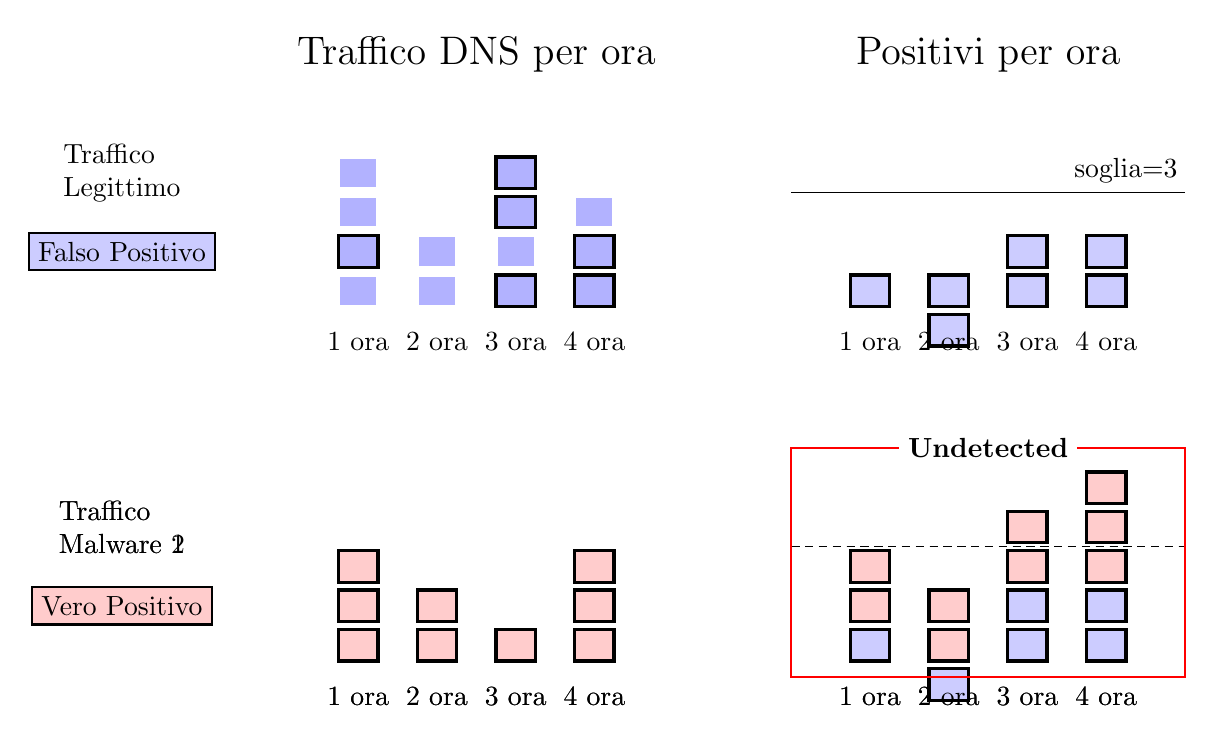
\begin{tikzpicture}

    \tikzset{
      pnode/.style={draw,minimum width=5mm,minimum height=4mm}
    }
    % \pic {ggrid};

    \def\neg{{0,1,0,0},{0,0},{1,0,1,1},{1,1,0}};
    \def\pos{{1,0,1},{1},{},{1,1,1}}
    \def\pn{1/2,0/1,3/0,2/3}

    \node[font=\Large] at ( 2, 3.5) {Traffico DNS per ora};
    \node[font=\Large] at (8.5, 3.5) {Positivi per ora};
    % \node[draw=white,thick,fill=blue!20] at ( 4, 3.5) {Vero Negativo};
    \node[draw,thick,fill=blue!20] at ( -2.5, 1) {Falso Positivo};
    % \node[draw=white,thick,fill=red!20] at ( 8, 3.5) {Falso Negativo};
    \onslide<3->{
      \node[draw,thick,fill=red!20] at ( -2.5, -3.5) {Vero Positivo};
    }

    \begin{scope}[xshift=0cm]
      \node[align=left] at (-2.5,2) {Traffico\\Legittimo};
      \foreach[count=\i] \arr in \neg {
        \foreach[count=\j] \x in \arr {
          \pgfmathsetmacro{\c}{\x == 0 ? "white" : "black"}
          \node[fill=blue!30,draw=\c,very thick,pnode] (n\i\j) at (\i-0.5,\j*5mm) {};
        }
        \node at (\i-0.5, -0.15) {\i\ ora};
      }

      \onslide<2->{
        \begin{scope}[xshift=6cm]
        \foreach[count=\i] \fp in {1,0,2,2} {
          \ifthenelse{\fp>0}{
            \foreach \j in {1,...,\fp} {
              \node[fill=blue!20,draw=black,very thick,pnode] (pp\i\j) at (\i,\j*5mm) {};
            }
          }{}
          \node at (\i, -0.15) {\i\ ora};
        }
        \draw [] (0,17.5mm) -- (5,17.5mm) node[above,pos=0.85] {soglia=3};
      \end{scope}
      }
    \end{scope}


    \begin{scope}[yshift=-4.5cm]
      \onslide<3-4>{
        \node[align=left] at (-2.5,2) {Traffico\\Malware 1};
        \foreach[count=\i] \arr in \pos {
          \foreach[count=\j] \x in \arr {
            \pgfmathsetmacro{\c}{\x == 0 ? "white" : "black"}
            \node[fill=red!20,draw=\c,very thick,pnode] (p\i\j) at (\i-0.5,\j*5mm) {};
          }
          \node at (\i-0.5, -0.15) {\i\ ora};
        }
      }

      \onslide<4>{
        \begin{scope}[xshift=6cm]
          \foreach[count=\i] \fp/\tp in \pn {
            \ifthenelse{\fp>0}{
              \foreach \j in {1,...,\fp} {
                \node[fill=blue!20,draw=black,very thick,pnode] (pp\i\j) at (\i,\j*5mm) {};
              }
            }{}
            \ifthenelse{\tp > 0}{
              \foreach \j in {1,...,\tp} {
                \pgfmathtruncatemacro{\jj}{\fp+\j}
                \node[fill=red!20,draw=black,very thick,pnode] (pp\i\jj) at (\i,\jj*5mm) {};
              }
            }{}
            \node at (\i, -0.15) {\i\ ora};
          }
          % \draw [dashed] (0,22.5mm) -- (5,22.5mm);
          \draw [densely dashed] (0,17.5mm) -- (5,17.5mm);
          \draw[ForestGreen,thick] (0, 0.1) rectangle (5, 3);
          \node[fill=white] at (2.5, 3) {\textbf{Detected}};
        \end{scope}
      }
    \end{scope}

    \def\neg{{0,1,0,0},{0,0},{0,1,0,1},{1,1,0,0}};
    \def\pos{{1,1},{1,1},{1},{1}}
    \def\pn{1/2,0/2,2/1,2/1}

    \begin{scope}[yshift=-4.5cm]
      \onslide<5-6>{
        \node[align=left] at (-2.5,2) {Traffico\\Malware 2};
        \foreach[count=\i] \arr in \pos {
          \foreach[count=\j] \x in \arr {
            \pgfmathsetmacro{\c}{\x == 0 ? "white" : "black"}
            \node[fill=red!20,draw=\c,very thick,pnode] (p\i\j) at (\i-0.5,\j*5mm) {};
          }
          \node at (\i-0.5, -0.15) {\i\ ora};
        }
      }

      \onslide<6>{
        \begin{scope}[xshift=6cm]
          \foreach[count=\i] \fp/\tp in \pn {
            \ifthenelse{\fp>0}{
              \foreach \j in {1,...,\fp} {
                \node[fill=blue!20,draw=black,very thick,pnode] (pp\i\j) at (\i,\j*5mm) {};
              }
            }{}
            \ifthenelse{\tp > 0}{
              \foreach \j in {1,...,\tp} {
                \pgfmathtruncatemacro{\jj}{\fp+\j}
                \node[fill=red!20,draw=black,very thick,pnode] (pp\i\jj) at (\i,\jj*5mm) {};
              }
            }{}
            \node at (\i, -0.15) {\i\ ora};
          }
          \draw [densely dashed] (0,17.5mm) -- (5,17.5mm);
          \draw[red,thick] (0, 0.1) rectangle (5, 3);
          \node[fill=white] at (2.5, 3) {\textbf{Undetected}};
        \end{scope}
      }
    \end{scope}
  \end{tikzpicture}%
  }
\end{center}
\end{frame}


\begin{frame}{Data set}


  \begin{center}
    \resizebox{\textwidth}{!}{%


    \begin{tikzpicture}

      \node at (-2,4) {%
      \parbox{9cm}{\begin{itemize}
        \item \ac{PCAP} da Stratosphere repository.
        \item Un tipo di traffico legittimo.
        \item Quattro diversi traffici malevoli.
        \begin{itemize}
          \item Malware \textit{caphaw}.
          \item Malware \textit{simda}.
          \item Malware \textit{virut}.
          \item Malware \textit{zbot}.
        \end{itemize}
      \end{itemize}}
      };

      \node[draw, rounded corners, text width=1.75cm] (lstm) at (4,4) {
\includegraphics[width=\textwidth]{ml.pdf}};
      \node[fill=white,font=\large] at (lstm.north) {\textbf{LSTM}};

      \node[text width=12cm] at (0,0) {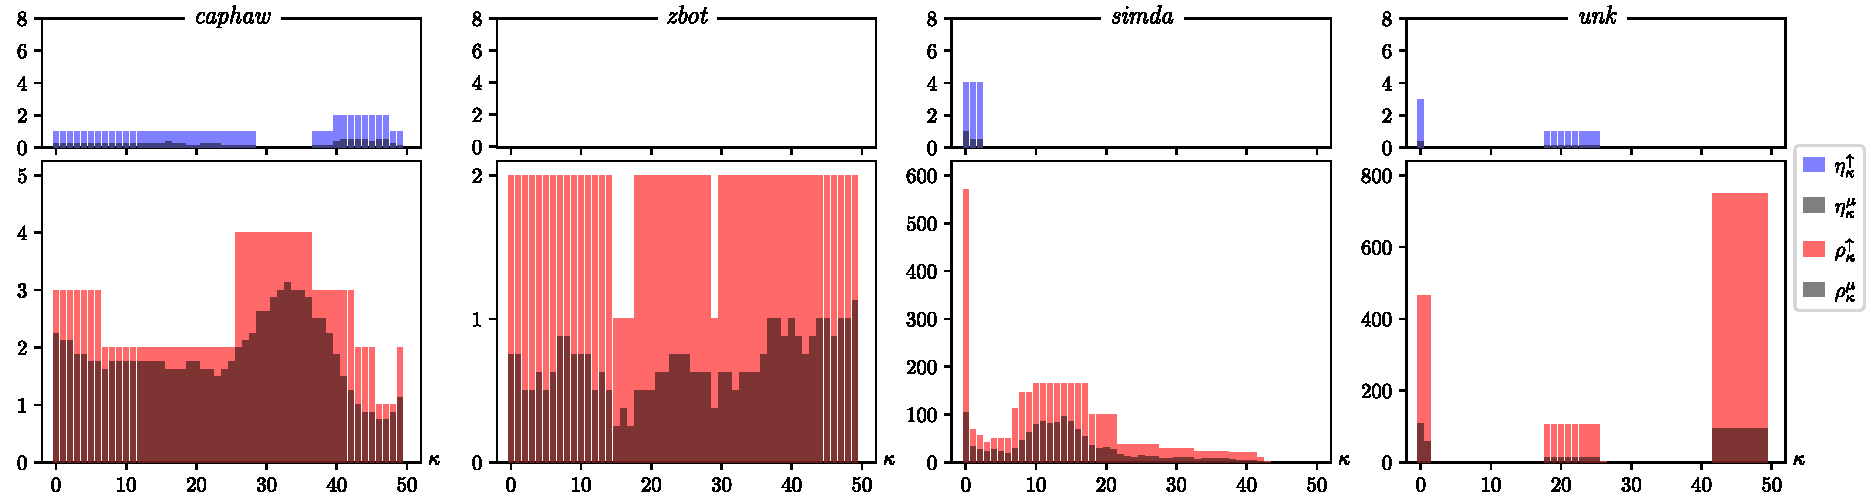
\includegraphics[width=1\textwidth]{malicious_s3.pdf}};
  \end{tikzpicture}
  }
\end{center}
\end{frame}


\begin{frame}{Conclusioni}
  \begin{center}
    \begin{tabular}{lllll}
      \textit{malware} & \phantom{ab} & TPR &\phantom{b} & \multicolumn{1}{p{3cm}}{Ore con attività malevola rilevate} \\\midrule
      caphaw      && 0.96 && 100\%    \\
      simda       && 0.95 && 86\%    \\
      virut       && 0.93 && 36\%    \\
      zbot        && 0.94 && 90\%    \\\bottomrule
    \end{tabular}
  \end{center}
  \begin{itemize}
    \item L'efficienza di rilevazione dipende dall'evoluzione temporale del traffico malevolo e benevolo.
    \item Necessario studio di una soglia dinamica.
    \item Necessario studio evoluzione temporale traffico benevolo e malevolo.
  \end{itemize}
\end{frame}

